% Flowchart: from a K-map / truth table to a quantum circuit, this work vs. tweedledum (PPRM, PKRM).
% Build: pdflatex flowchart.tex
\documentclass[border=8pt]{standalone}
\usepackage{amsmath,amssymb}
\usepackage{tikz}
\usetikzlibrary{positioning,arrows.meta,fit,backgrounds,calc}

\definecolor{ours}{RGB}{31,94,160}
\definecolor{tw}{RGB}{176,92,20}
\definecolor{shared}{RGB}{70,70,70}

\tikzset{
  box/.style={draw=#1, line width=0.9pt, rounded corners=4pt, fill=#1!6, align=left,
              text width=6.6cm, inner sep=6pt, font=\small},
  wide/.style={draw=shared, line width=0.9pt, rounded corners=4pt, fill=shared!6, align=left,
               text width=14.6cm, inner sep=6pt, font=\small},
  ex/.style={font=\footnotesize\itshape},
  arr/.style={-{Stealth[length=7pt]}, line width=1pt, draw=#1},
  head/.style={font=\bfseries\large, text=#1},
}
\newcommand{\step}[2]{\textbf{#1}\\[2pt]#2}

\begin{document}
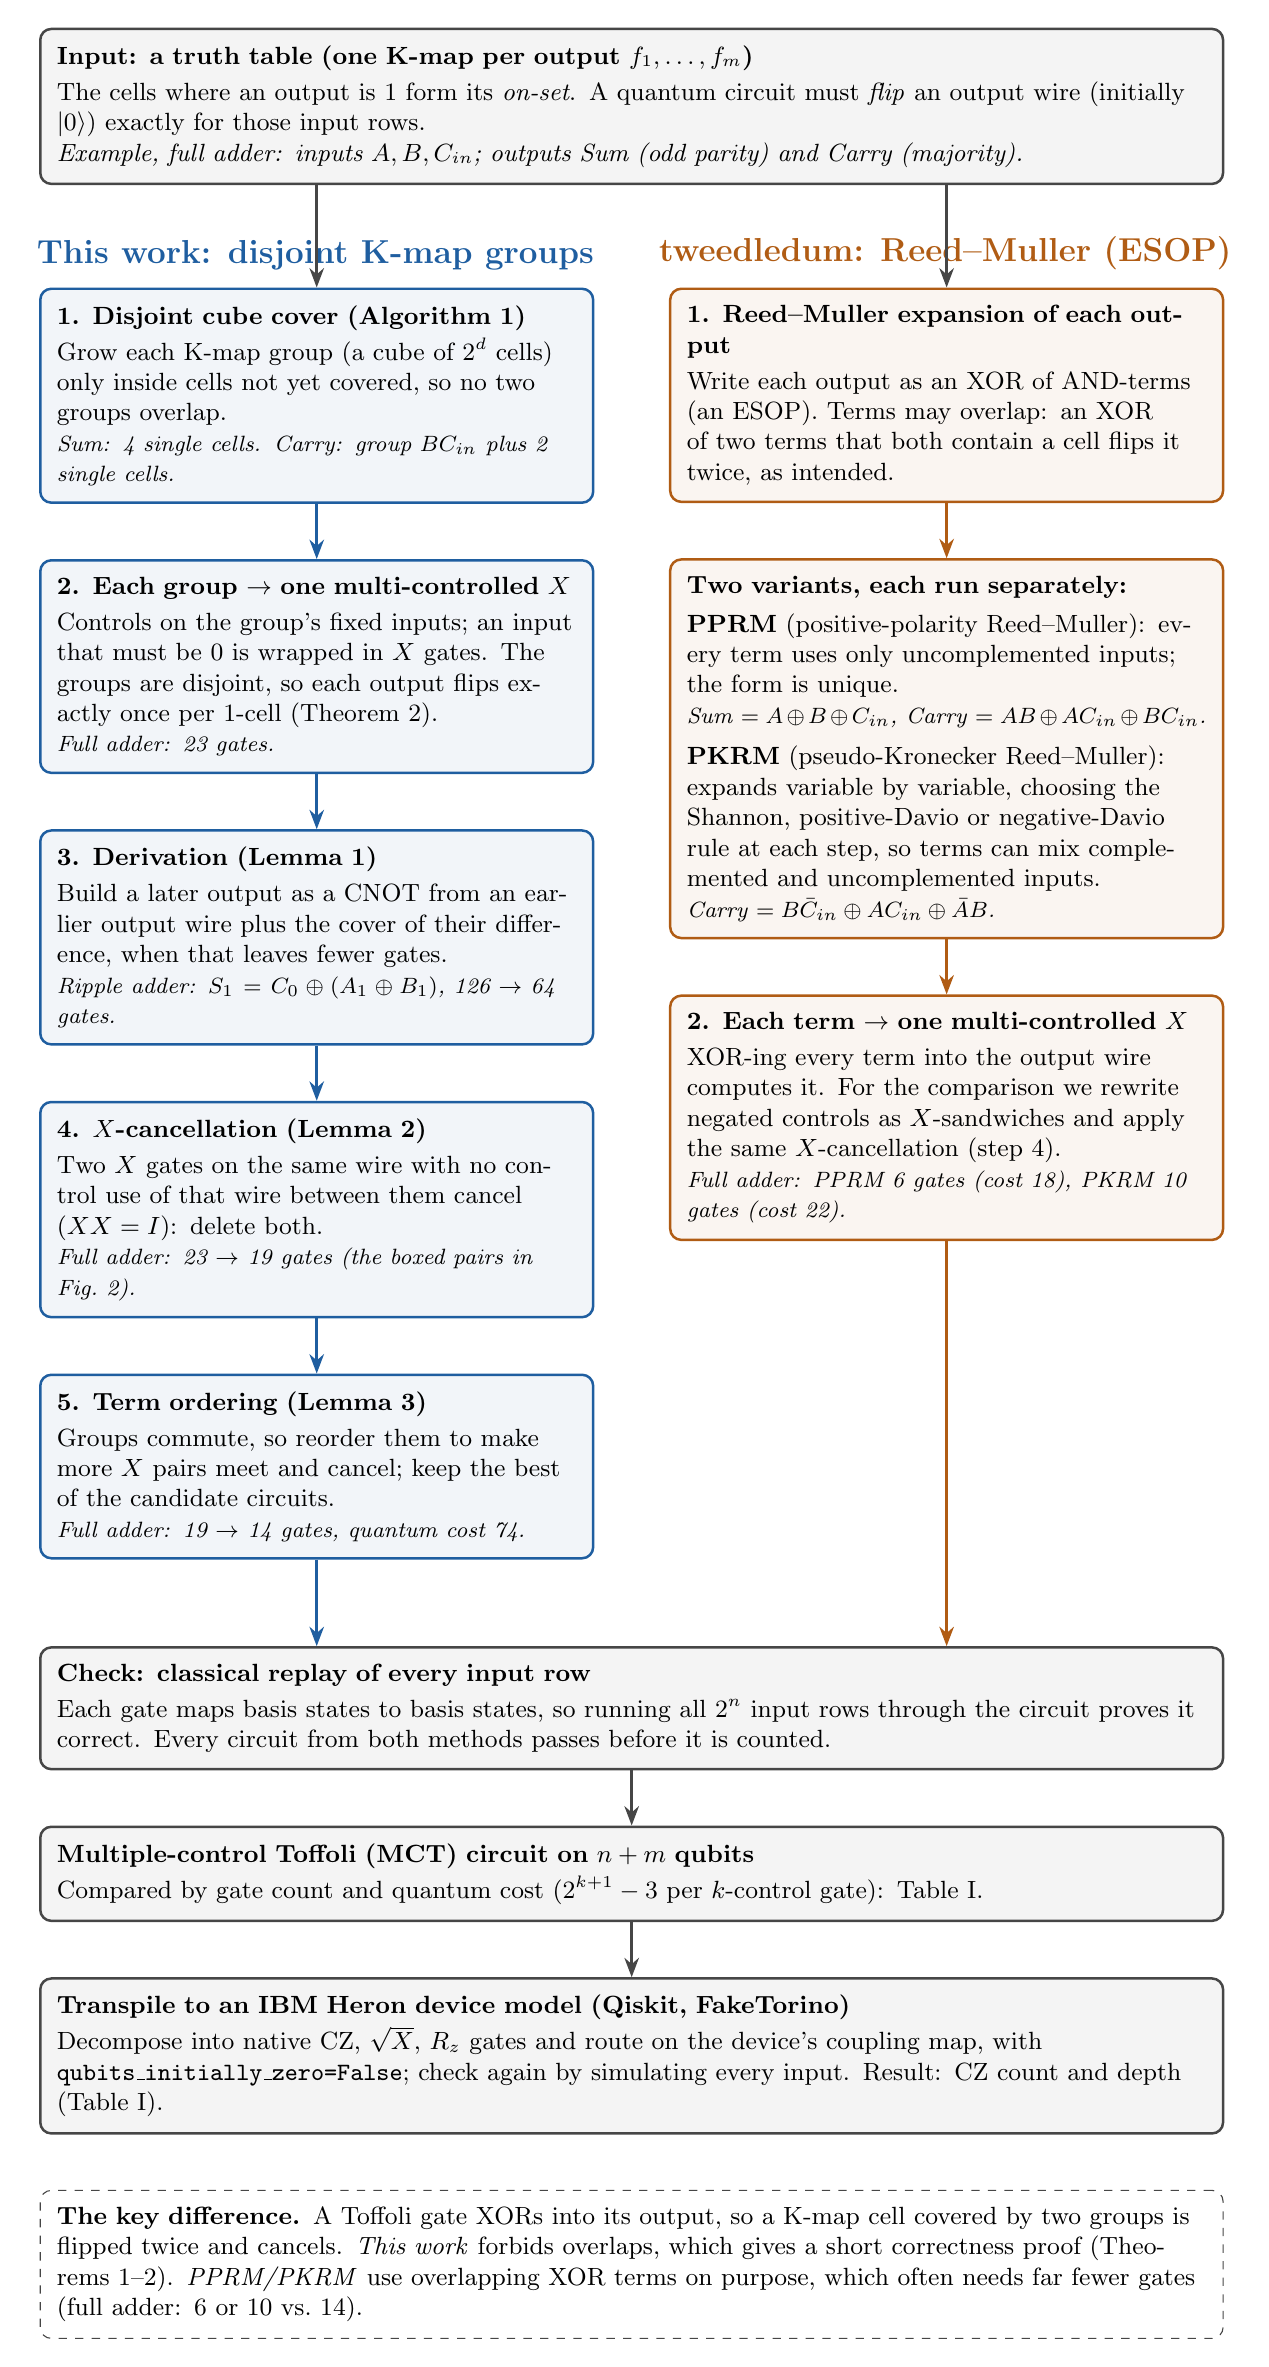
\begin{tikzpicture}[node distance=7mm]

% ---------------- input ----------------
\node[wide, anchor=north west] (in) at (0,0) {\step{Input: a truth table (one K-map per output $f_1,\dots,f_m$)}
  {The cells where an output is $1$ form its \emph{on-set}. A quantum circuit must \emph{flip} an
  output wire (initially $\lvert0\rangle$) exactly for those input rows.\\
  \textit{Example, full adder: inputs $A,B,C_{in}$; outputs Sum (odd parity) and Carry (majority).}}};

% column heads
% two columns, each 7.02cm wide (6.6cm text + padding), 0.98cm apart, under the 15.02cm wide boxes
\coordinate (L) at ($(in.south west)+(0,-1.3)$);
\coordinate (Rt) at ($(in.south west)+(8.0,-1.3)$);
\node[head=ours, anchor=south] (h1) at ($(L)+(3.51,0.1)$) {This work: disjoint K-map groups};
\node[head=tw, anchor=south] (h2) at ($(Rt)+(3.51,0.1)$) {tweedledum: Reed--Muller (ESOP)};

% ---------------- this work ----------------
\node[box=ours, anchor=north west] (a1) at (L) {\step{1. Disjoint cube cover (Algorithm 1)}
  {Grow each K-map group (a cube of $2^d$ cells) only inside cells not yet covered, so no two
  groups overlap.\\
  {\footnotesize\itshape Sum: 4 single cells. Carry: group $BC_{in}$ plus 2 single cells.}}};

\node[box=ours, below=of a1] (a2) {\step{2. Each group $\to$ one multi-controlled $X$}
  {Controls on the group's fixed inputs; an input that must be $0$ is wrapped in $X$ gates. The
  groups are disjoint, so each output flips exactly once per $1$-cell (Theorem 2).\\
  {\footnotesize\itshape Full adder: 23 gates.}}};

\node[box=ours, below=of a2] (a3) {\step{3. Derivation (Lemma 1)}
  {Build a later output as a CNOT from an earlier output wire plus the cover of their
  difference, when that leaves fewer gates.\\
  {\footnotesize\itshape Ripple adder: $S_1 = C_0 \oplus (A_1\oplus B_1)$, 126 $\to$ 64 gates.}}};

\node[box=ours, below=of a3] (a4) {\step{4. $X$-cancellation (Lemma 2)}
  {Two $X$ gates on the same wire with no control use of that wire between them cancel
  ($XX=I$): delete both.\\
  {\footnotesize\itshape Full adder: 23 $\to$ 19 gates (the boxed pairs in Fig.~2).}}};

\node[box=ours, below=of a4] (a5) {\step{5. Term ordering (Lemma 3)}
  {Groups commute, so reorder them to make more $X$ pairs meet and cancel; keep the best of
  the candidate circuits.\\
  {\footnotesize\itshape Full adder: 19 $\to$ 14 gates, quantum cost 74.}}};

% ---------------- tweedledum ----------------
\node[box=tw, anchor=north west] (b1) at (Rt) {\step{1. Reed--Muller expansion of each output}
  {Write each output as an XOR of AND-terms (an ESOP). Terms may overlap: an XOR of two
  terms that both contain a cell flips it twice, as intended.}};
\node[box=tw, below=of b1] (b2) {\textbf{Two variants, each run separately:}\\[3pt]
  \textbf{PPRM} (positive-polarity Reed--Muller): every term uses only uncomplemented inputs;
  the form is unique.\\
  {\footnotesize\itshape Sum $= A\oplus B\oplus C_{in}$,\ Carry $= AB\oplus AC_{in}\oplus BC_{in}$.}\\[4pt]
  \textbf{PKRM} (pseudo-Kronecker Reed--Muller): expands variable by variable, choosing the
  Shannon, positive-Davio or negative-Davio rule at each step, so terms can mix complemented
  and uncomplemented inputs.\\
  {\footnotesize\itshape Carry $= B\bar C_{in}\oplus AC_{in}\oplus \bar A B$.}};
\node[box=tw, below=of b2] (b4) {\step{2. Each term $\to$ one multi-controlled $X$}
  {XOR-ing every term into the output wire computes it. For the comparison we rewrite negated
  controls as $X$-sandwiches and apply the same $X$-cancellation (step 4).\\
  {\footnotesize\itshape Full adder: PPRM 6 gates (cost 18), PKRM 10 gates (cost 22).}}};

% ---------------- shared tail ----------------
\node[wide, below=11mm of a5.south west, anchor=north west] (c1) {\step{Check: classical replay of every input row}
  {Each gate maps basis states to basis states, so running all $2^n$ input rows through the
  circuit proves it correct. Every circuit from both methods passes before it is counted.}};
\node[wide, below=of c1] (c2) {\step{Multiple-control Toffoli (MCT) circuit on $n+m$ qubits}
  {Compared by gate count and quantum cost ($2^{k+1}-3$ per $k$-control gate): Table I.}};
\node[wide, below=of c2] (c3) {\step{Transpile to an IBM Heron device model (Qiskit, FakeTorino)}
  {Decompose into native CZ, $\sqrt{X}$, $R_z$ gates and route on the device's coupling map, with
  \texttt{qubits\_initially\_zero=False}; check again by simulating every input.
  Result: CZ count and depth (Table I).}};

% ---------------- arrows ----------------
\draw[arr=shared] (in.south -| a1.north) -- (a1.north);
\draw[arr=shared] (in.south -| b1.north) -- (b1.north);
\foreach \u/\v in {a1/a2,a2/a3,a3/a4,a4/a5} \draw[arr=ours] (\u) -- (\v);
\draw[arr=tw] (b1) -- (b2);
\draw[arr=tw] (b2) -- (b4);
\draw[arr=ours] (a5.south) -- (a5.south |- c1.north);
\draw[arr=tw] (b4.south) -- (b4.south |- c1.north);
\draw[arr=shared] (c1) -- (c2);
\draw[arr=shared] (c2) -- (c3);

% ---------------- key difference ----------------
\node[draw=shared, dashed, rounded corners=4pt, align=left, text width=14.6cm, inner sep=6pt,
      font=\small, below=7mm of c3] (key) {\textbf{The key difference.} A Toffoli gate XORs into its
  output, so a K-map cell covered by two groups is flipped twice and cancels. \emph{This work}
  forbids overlaps, which gives a short correctness proof (Theorems 1--2). \emph{PPRM/PKRM} use
  overlapping XOR terms on purpose, which often needs far fewer gates (full adder: 6 or 10 vs.\ 14).};

\end{tikzpicture}
\end{document}
